\documentclass{article}
\usepackage{graphicx} % Required for inserting images
\usepackage{geometry}
\usepackage{wrapfig}
 \geometry{
 a4paper,
 total = {198mm,295mm},
 left = 2cm,
 right = 2cm,
 top = 2cm,
 bottom = 2cm
 }
\title{Mie holography and optical trapping to study colloid-colloid interaction}
\author{guirec de tournemire}
\date{July 21th 2026}

\begin{document}

\maketitle

\section{Experimental Method}
The method used to monitor the interaction between of two brownian particles is known as \textit{Mie Holography} \cite{lee2007characterizing,lavaud2021stochastic}. This method relies on the holograms produced by interferences between the incident light illuminating a particle, and the light scattered by the latter (see Fig. \ref{fig:scheme_Mie}a). The interferences patterns are extracted as intensity profiles (see Fig. \ref{fig:scheme_Mie}b) and fitted based on the Lorenz-Mie theory to recover the tridimensional position of the particle, for every frame composing the video. 

The sample consists of two glass slides (thickness $e=0.13-0.17 \, \mathrm{mm}$ and refractive index $n_\mathrm{g}=1.518)$) separated by paraffin bands. The space $H$ between the two glass slides, set by the thickness of the paraffin bands, is about $H = 250 \, \mathrm{\mu m}$. The Brownian microparticles are made of polystyrene, manufactured by Polyscience. They are negatively surface-charged and have a radius $a_\mathrm{p} = 1.5 \, \mathrm{\mu m}$, for a density of $\rho_p = 1050 \, \mathrm{g/cm^3}$. Their motion is recorded through a x100 oil-immersion Olympus objective (NA = 1.45), configured for TIRFM, using a Basler Camera, with a field of view of 70 $\times$ 70~$\mu$m in the $xOy$ plane. Along $z$, the depth of view $h$ is about $100 \, \mathrm{\mu m}$. The motion of the particles is recorded at a frequency $f=\frac{1}{dt}=200 \, \mathrm{Hz}$, leaving a lag time of $dt = 5 \, \mathrm{ms}$ between two frames.

\begin{figure}[h!]
    \centering
    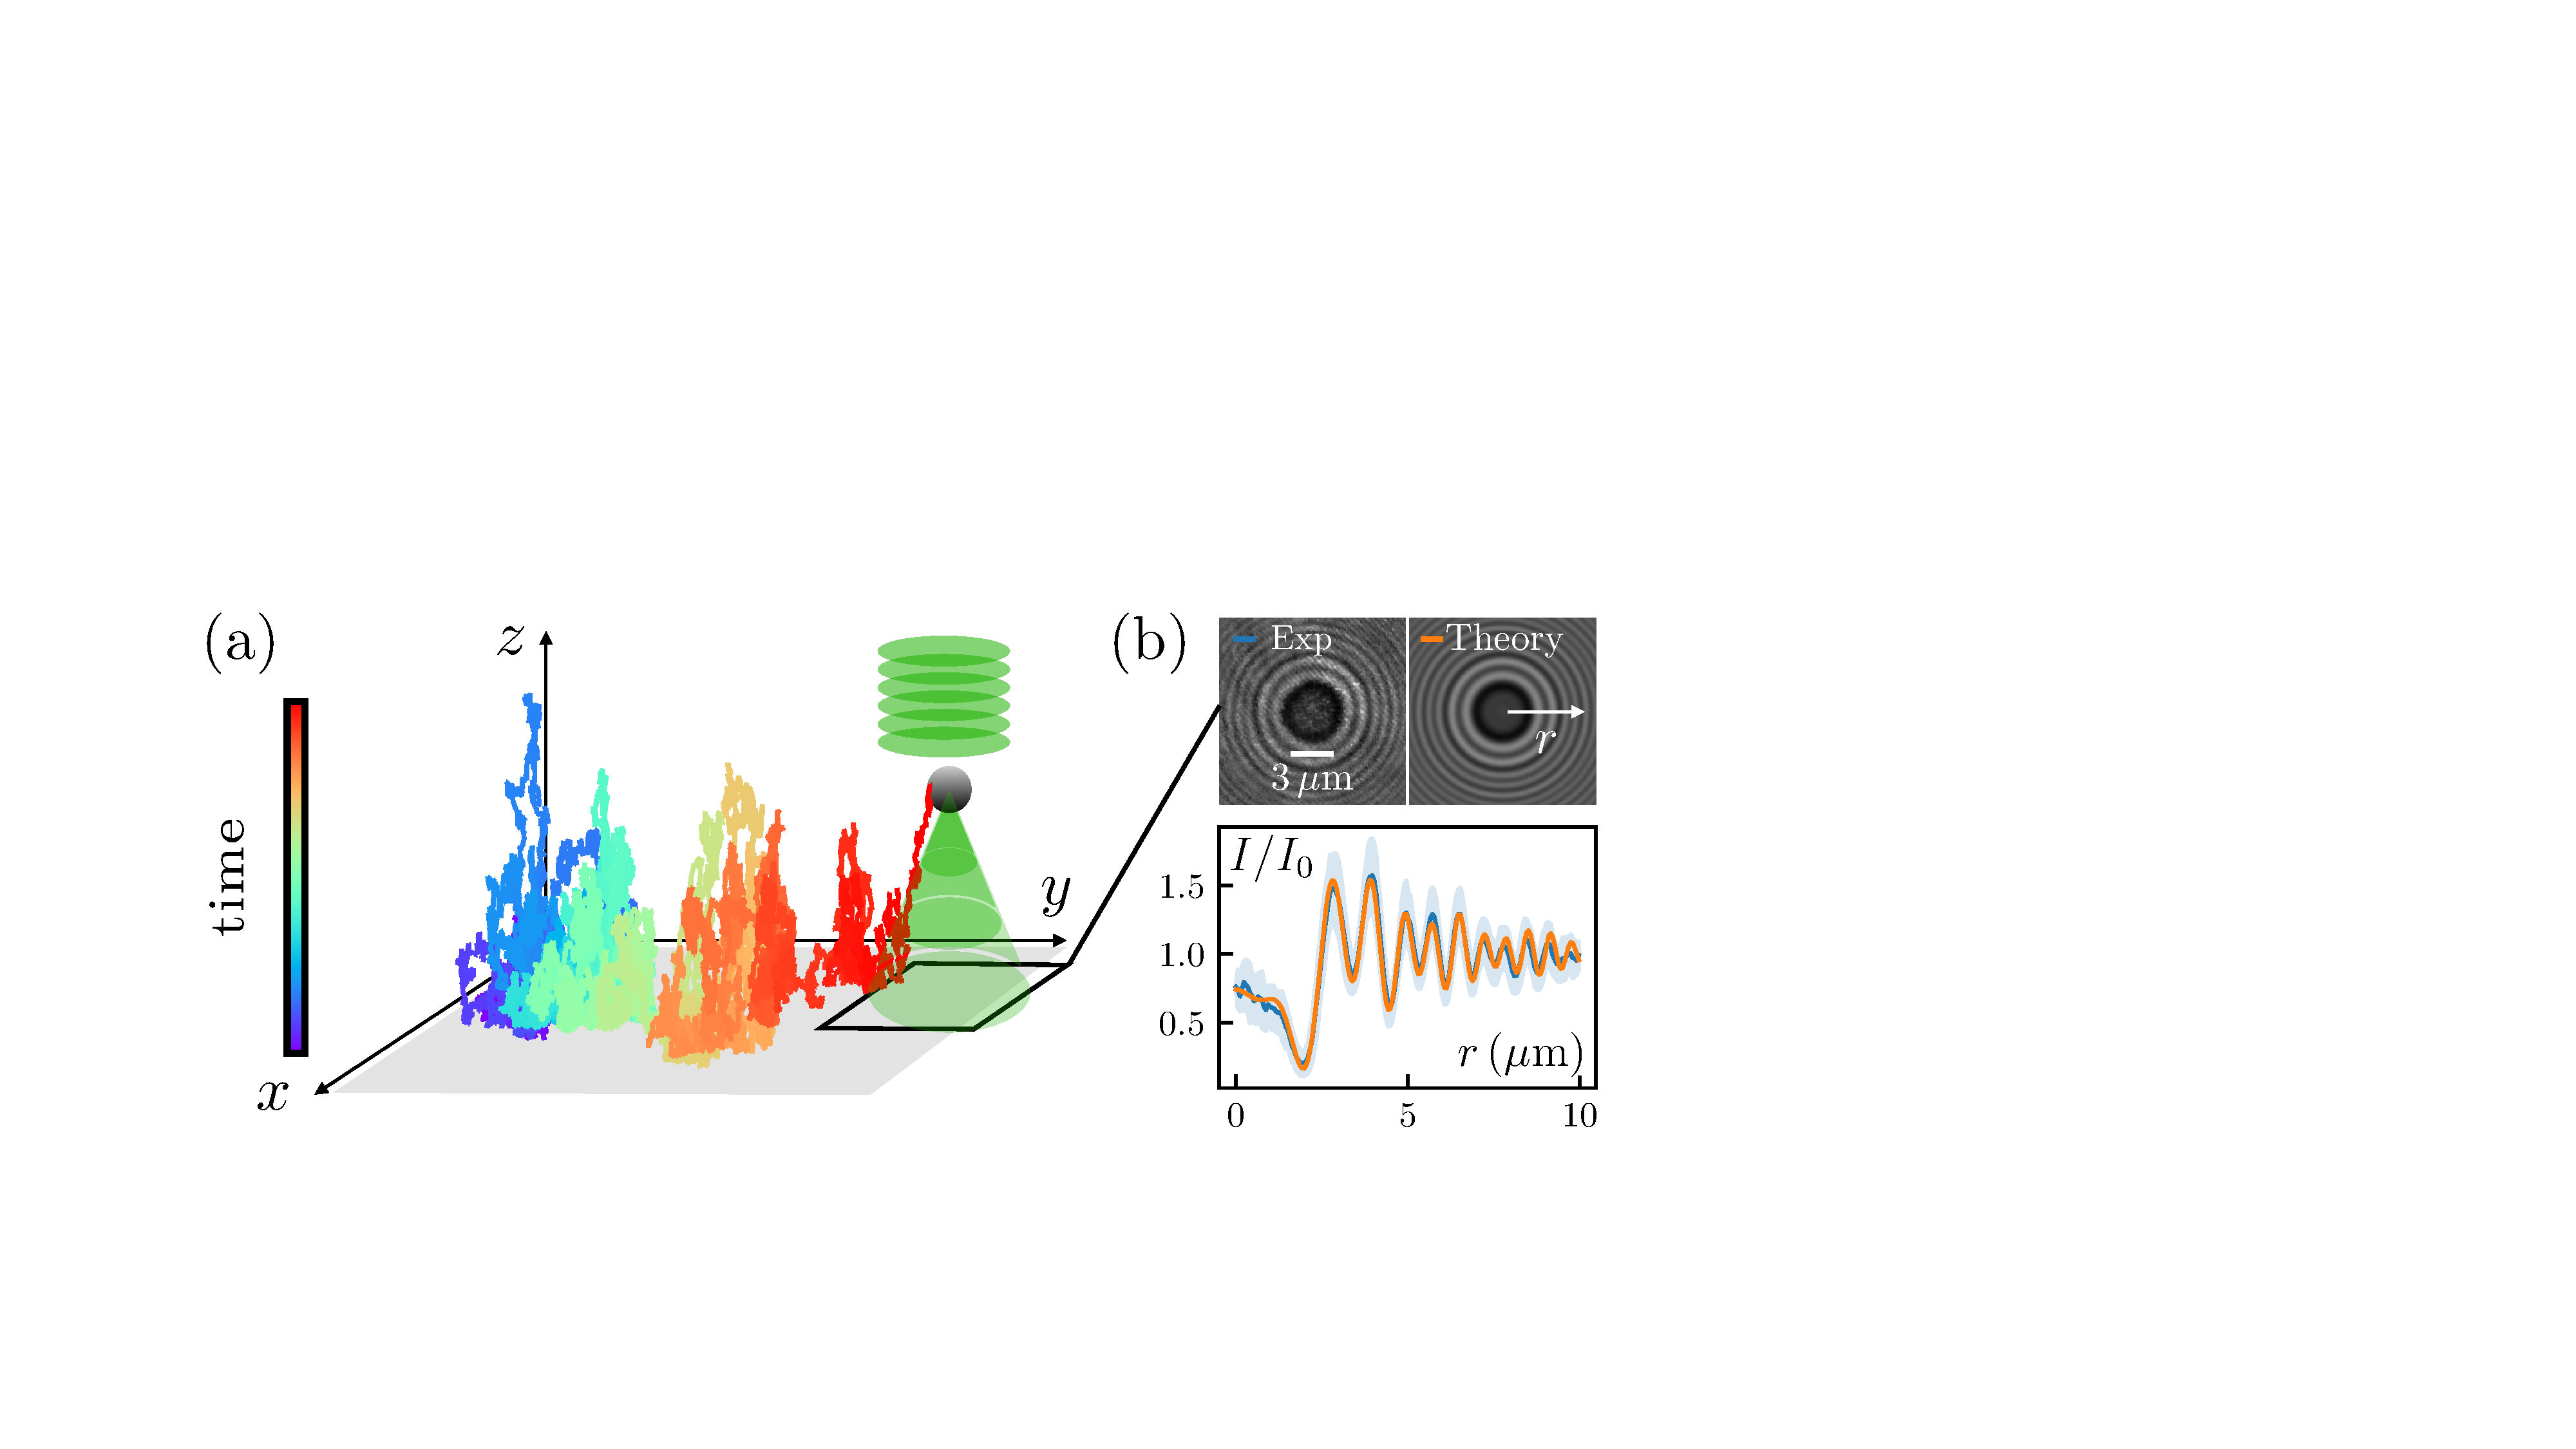
\includegraphics[width=0.45\linewidth]{Fig1.pdf}
    \caption{Mie Holography method used to probe the motion of a colloid $1.5 \, \mathrm{\mu m}$-radius particles in water, illuminated by a laser at $532 \, \mathrm{nm}$ at a laser power of $4 \, \mathrm{mW}$.}
    \label{fig:scheme_Mie}
\end{figure}





In order to enforce the hydrodynamic interaction between two particles, we set a \textit{optical trap} \cite{ashkin1992forces} , enabling the translation of a particle from one point to an other (see Fig. \ref{fig:scheme_trap}) . The method consist of finding a diffusing particle, move it as close as possible to another one, and take a video with a high frame rate to have as much data as possible, in the region where the particle-particle interaction is omnipresent.

\begin{figure}[h!]
    \centering
    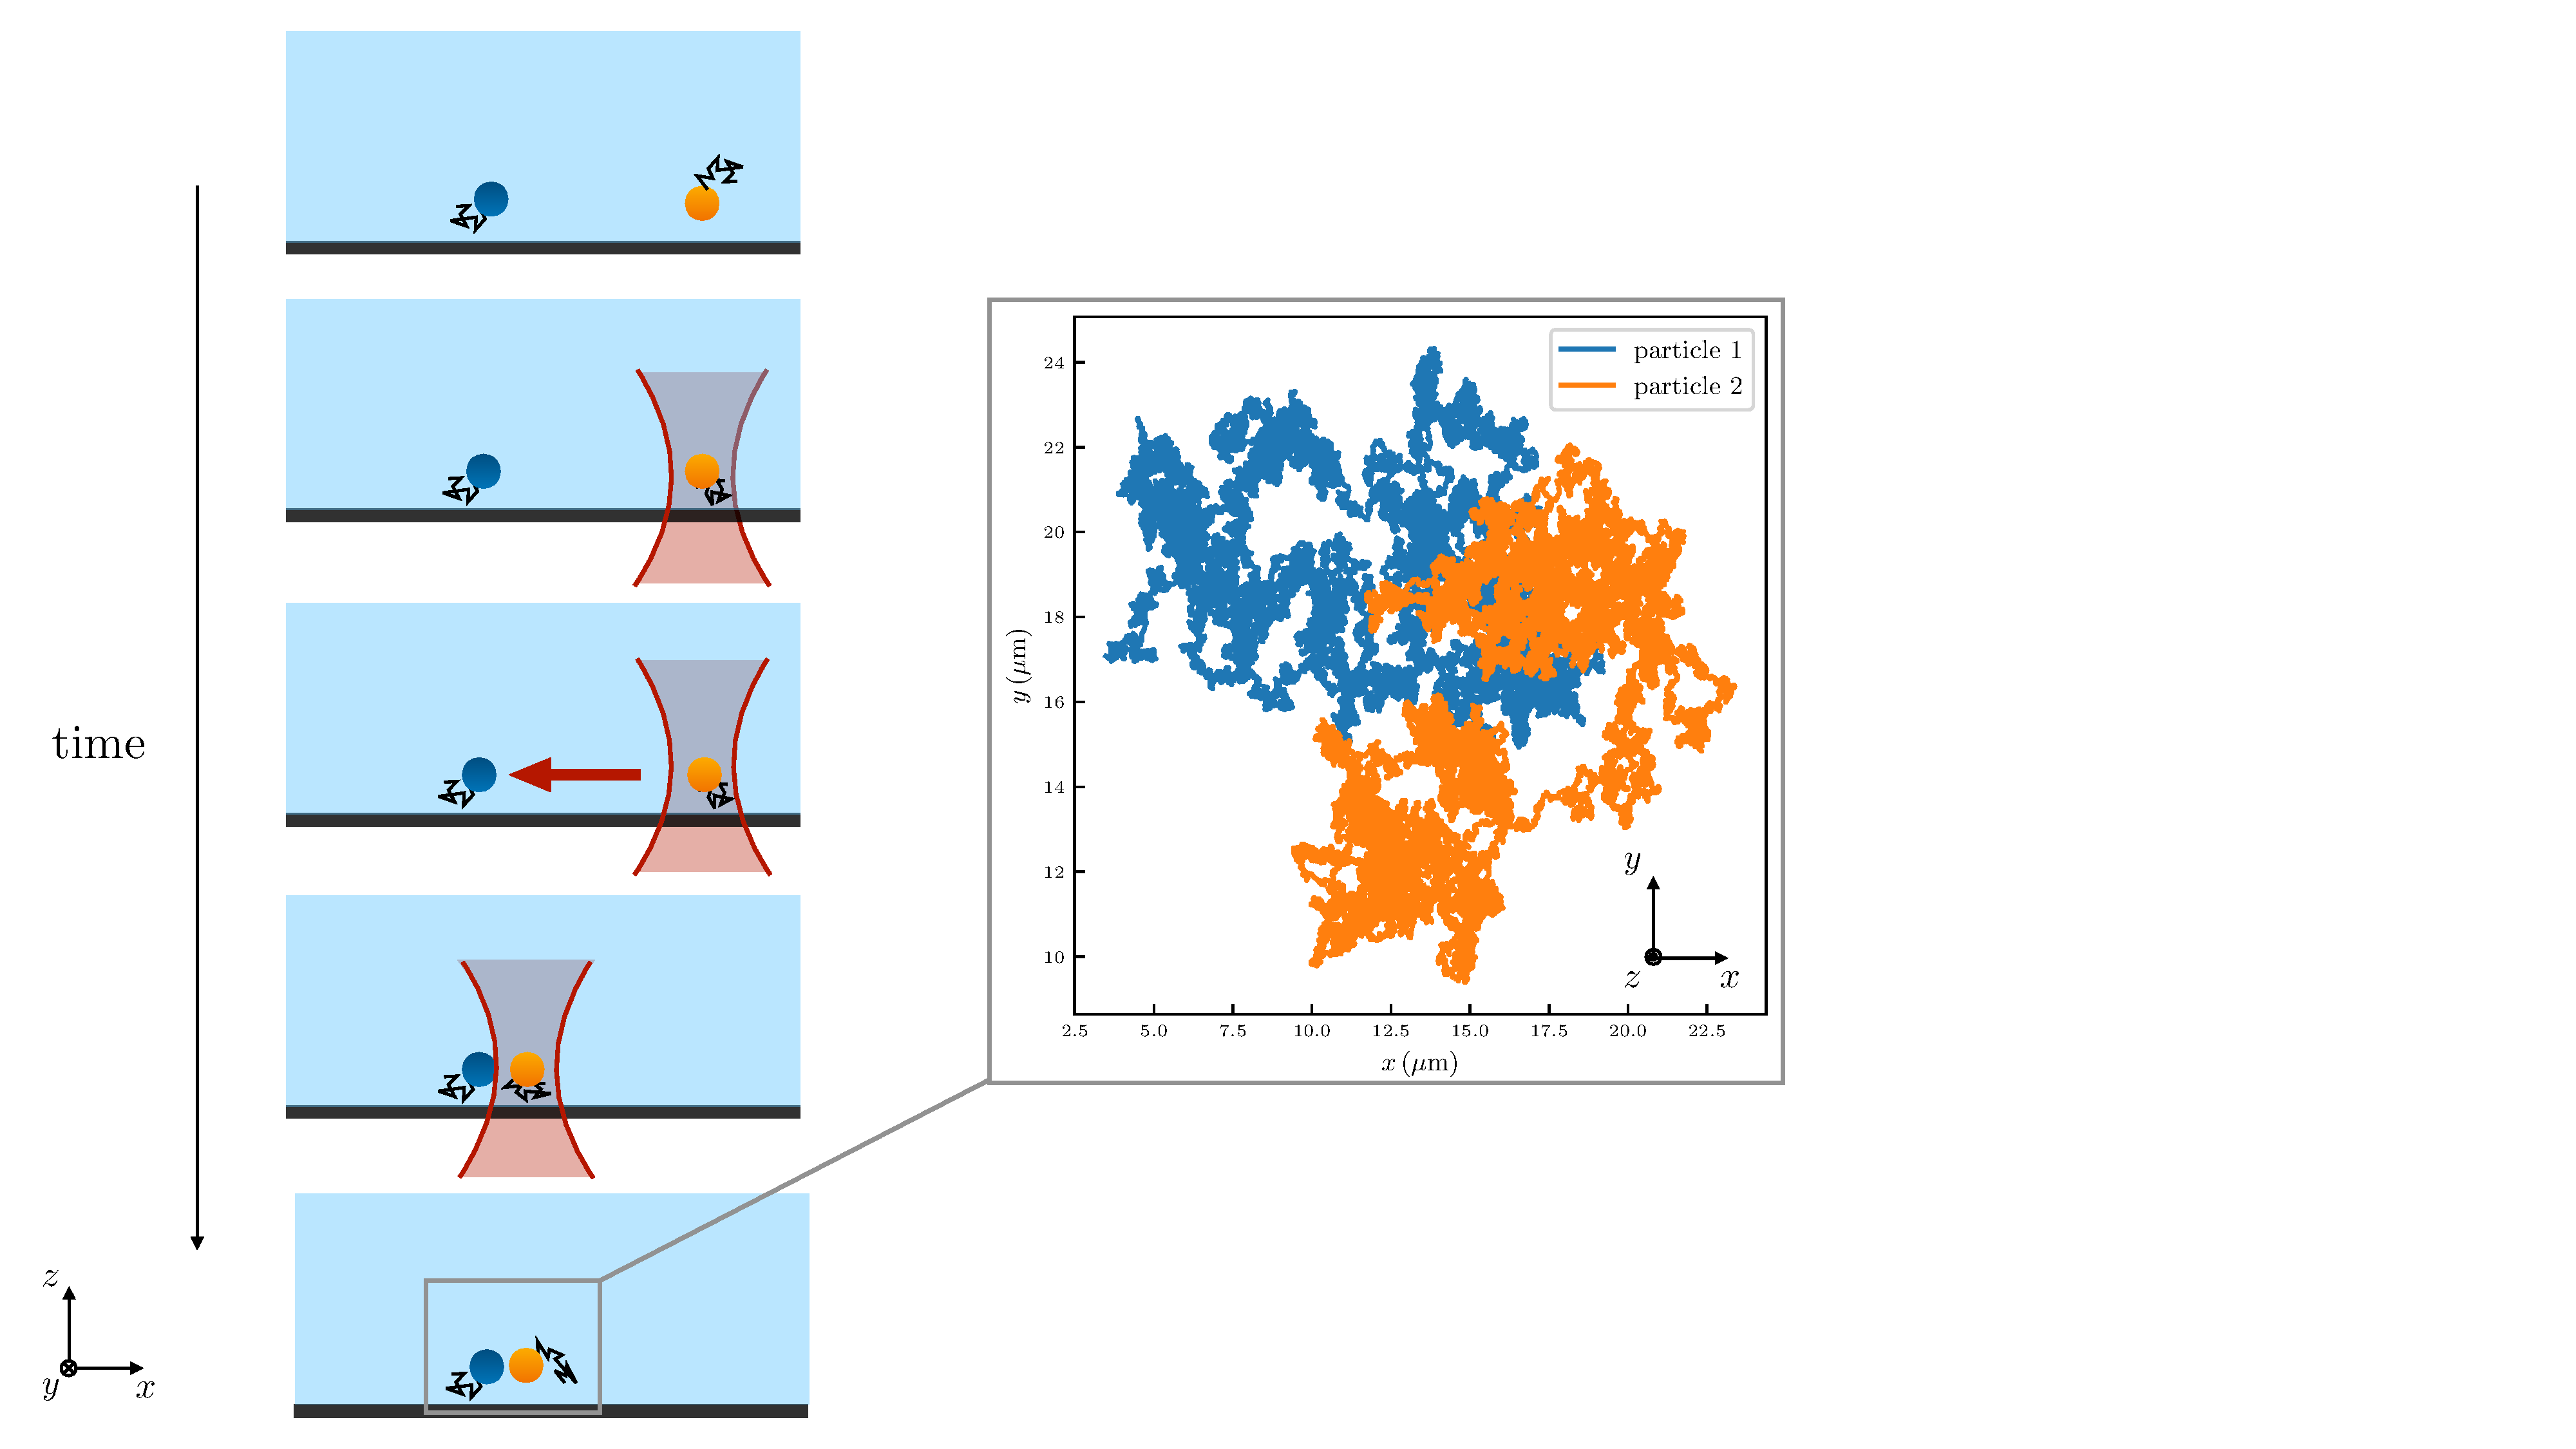
\includegraphics[width = 0.6\linewidth]{Fig2.pdf}
    \caption{Optical trapping used to enforce the colloid-colloid interaction. The trap is set by a laser at $660 \, \mathrm{nm}$ at a laser power of $50 \, \mathrm{mW}$.}
    \label{fig:scheme_trap}
\end{figure}



\bibliographystyle{ieeetr}
{\bibliography{references.bib}
}\end{document}
